\subsection{Realism analysis}

A t-SNE analysis, for \emph{t-distributed stochastic neighbor embedding}, of
the generated mixed-reality images and real images captured from the UAV's
camera, is given as a comparison in figure~\ref{fig:tsne}.

\begin{figure}[h!]
	\centering
	\begin{subfigure}[h]{0.49\textwidth}
		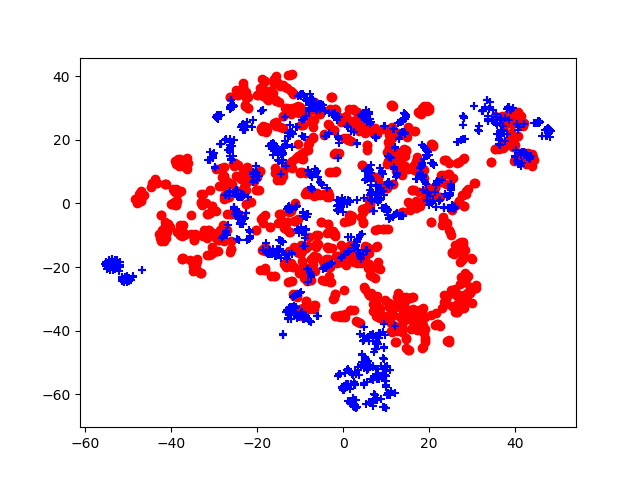
\includegraphics[width=\textwidth]{figure/tsne-2D.png}
		\caption{2D plot}
	\end{subfigure}
	\begin{subfigure}[h]{0.49\textwidth}
		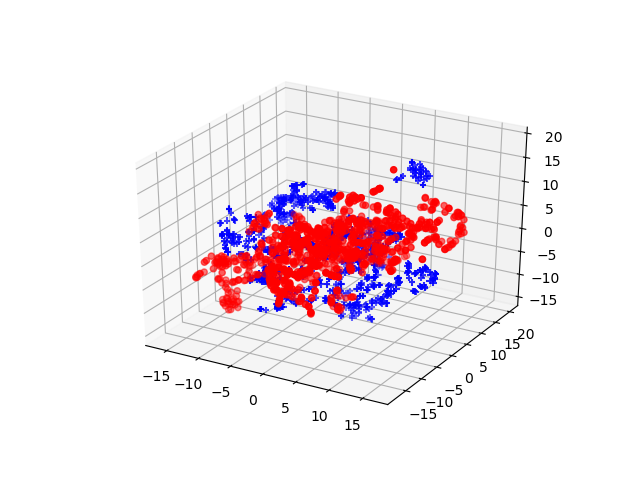
\includegraphics[width=\textwidth]{figure/tsne-3D.png}
		\caption{3D plot}
	\end{subfigure}
	\caption[T-SNE analysis of synthetic versus real images.]{T-SNE analysis of
	synthetic versus real images. The red labels represent the synthetic
	images, while the blue labels show the real ones.} \label{fig:tsne}
\end{figure}

This dimensionality reduction technique is very useful to visualize high
dimensional data such as images. The $640 \times 480$ images used for
comparison are so dimensionaly high that PCA (Principal Component Analysis)
needs to be applied first, otherwise the t-SNE algorithm would be too sensitive
to noise, and the computation of pairwise distances between the samples would
be too slow.\\

Several small clusters can be observed on the plots, which means there are
disparities between the real and fake images. To push the analysis further and
attempt to explain the origin of this clustering, a few samples in those
regions are shown, and conclusions are drawn.

\textcolor{red}{Add 3x2 matrix of images to compare real vs fake gates.}


\begin{figure}[h!]
	\centering
	\begin{subfigure}{0.35\textwidth}
		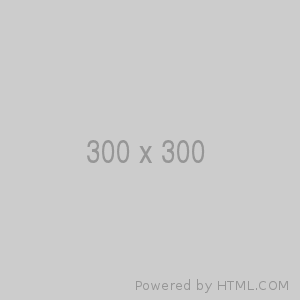
\includegraphics[width=\textwidth]{figure/300x300.png}
	\end{subfigure}
	\begin{subfigure}{0.35\textwidth}
		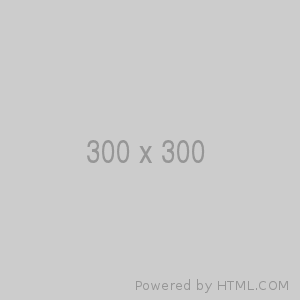
\includegraphics[width=\textwidth]{figure/300x300.png}
	\end{subfigure}
	\begin{subfigure}{0.35\textwidth}
		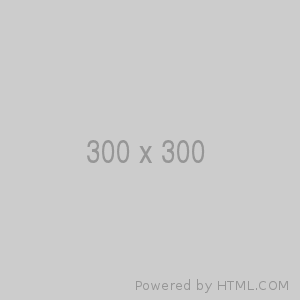
\includegraphics[width=\textwidth]{figure/300x300.png}
	\end{subfigure}
	\begin{subfigure}{0.35\textwidth}
		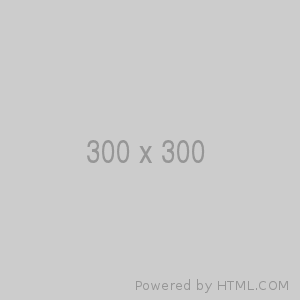
\includegraphics[width=\textwidth]{figure/300x300.png}
	\end{subfigure}
	\begin{subfigure}{0.35\textwidth}
		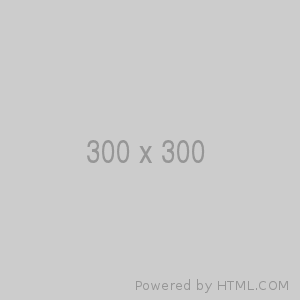
\includegraphics[width=\textwidth]{figure/300x300.png}
	\end{subfigure}
	\begin{subfigure}{0.35\textwidth}
		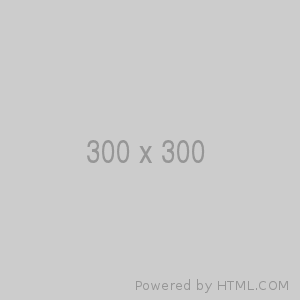
\includegraphics[width=\textwidth]{figure/300x300.png}
	\end{subfigure}
	\caption[Synthetic versus real images comparison]{}
\end{figure}

\textcolor{red}{Explain why each sample belongs to a different cluster.}


Furthermore, this analysis is made on a random selection of samples, which is
not well balanced due to the fact that each batch of synthetic images shows
roughly 70\% of gates visibility, while the real test set -- being a lot less
random -- is probably closer to 100\%. To get rid of these disparities and
offer a fairer comparison, another t-SNE analysis, this time applied to
hand-picked samples, is shown in figure~\ref{fig:tsne-manual}. Those manually
selected samples represent similar configurations of gate placement, and intend
to eliminate cases where no gates are visible.

\begin{figure}[h!]
	\centering
	\begin{subfigure}[h]{0.49\textwidth}
		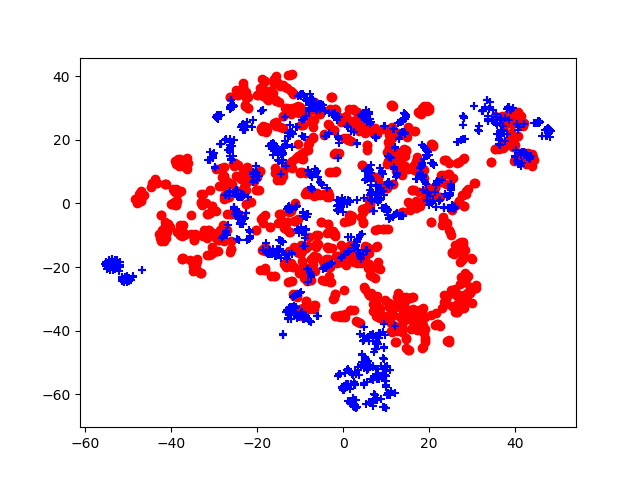
\includegraphics[width=\textwidth]{figure/tsne-2D.png}
		\caption{2D plot}
	\end{subfigure}
	\begin{subfigure}[h]{0.49\textwidth}
		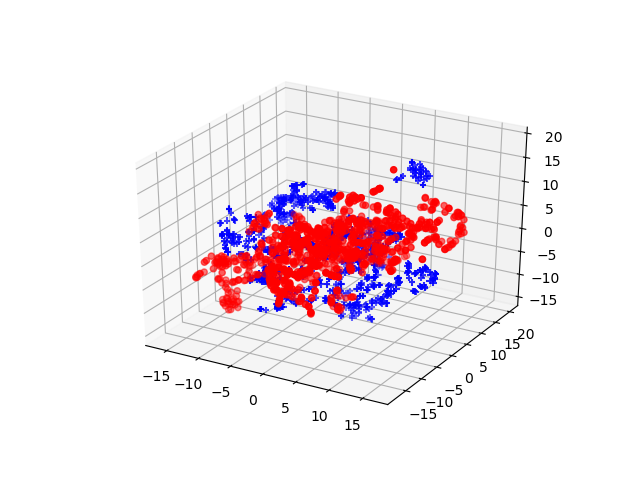
\includegraphics[width=\textwidth]{figure/tsne-3D.png}
		\caption{3D plot}
	\end{subfigure}
	\caption[T-SNE analysis of hand-picked samples.]{T-SNE analysis of
	manually selected samples of synthetic and real images. The red labels
	represent the synthetic images, while the blue labels show the real ones.}
	\label{fig:tsne-manual}
\end{figure}

\textcolor{red}{Conclude on this proper analysis, and also add a 3x2 matrix
of image samples}.

\newpage

\begin{figure}[h!]
	\centering
	\begin{subfigure}{0.35\textwidth}
		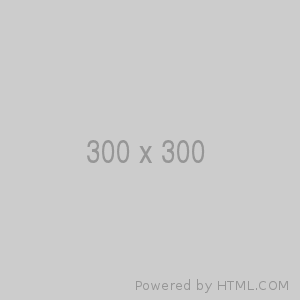
\includegraphics[width=\textwidth]{figure/300x300.png}
	\end{subfigure}
	\begin{subfigure}{0.35\textwidth}
		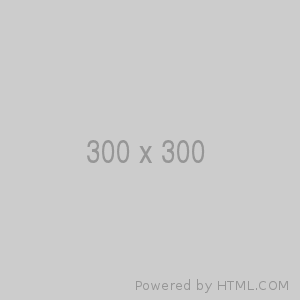
\includegraphics[width=\textwidth]{figure/300x300.png}
	\end{subfigure}
	\begin{subfigure}{0.35\textwidth}
		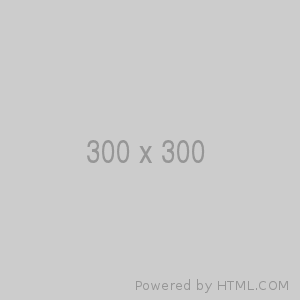
\includegraphics[width=\textwidth]{figure/300x300.png}
	\end{subfigure}
	\begin{subfigure}{0.35\textwidth}
		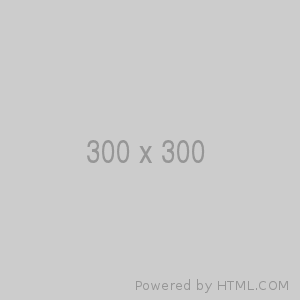
\includegraphics[width=\textwidth]{figure/300x300.png}
	\end{subfigure}
	\begin{subfigure}{0.35\textwidth}
		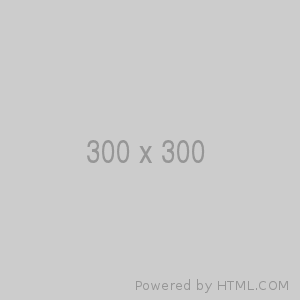
\includegraphics[width=\textwidth]{figure/300x300.png}
	\end{subfigure}
	\begin{subfigure}{0.35\textwidth}
		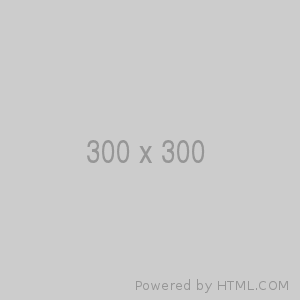
\includegraphics[width=\textwidth]{figure/300x300.png}
	\end{subfigure}
	\caption[Synthetic versus real images comparison]{}
\end{figure}

~\\Overall, the generation of synthetic gates can be considered a success, as
it is not obvious whether an image comes from the synthetic dataset or the real
test dataset, in some cases. Naturally, a subjective opinion is not enough to
confirm the viability of the obtained results, and the t-SNE analysis provides
the additional arguments to lean on this hypothesis.
\newpage
